% Eixos previstos abaixo da grade; títulos alinhados no topo dos painéis.
\begin{minipage}[t]{.48\linewidth}\centering
\textbf{Escopo (550 OOF)}\par
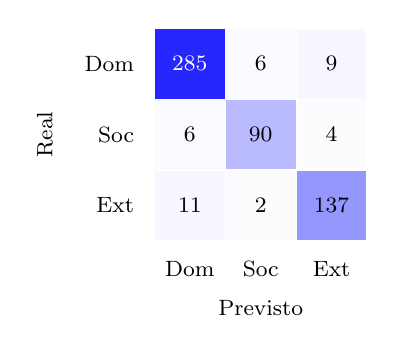
\begin{tikzpicture}[x=.90cm,y=.90cm,font=\footnotesize]
\filldraw[fill=blue!85,draw=white] (0,2) rectangle (1,3);
\node[text=white] at (0.5,2.5) {285};
\filldraw[fill=blue!2,draw=white] (1,2) rectangle (2,3);
\node[text=black] at (1.5,2.5) {6};
\filldraw[fill=blue!3,draw=white] (2,2) rectangle (3,3);
\node[text=black] at (2.5,2.5) {9};
\filldraw[fill=blue!2,draw=white] (0,1) rectangle (1,2);
\node[text=black] at (0.5,1.5) {6};
\filldraw[fill=blue!27,draw=white] (1,1) rectangle (2,2);
\node[text=black] at (1.5,1.5) {90};
\filldraw[fill=blue!1,draw=white] (2,1) rectangle (3,2);
\node[text=black] at (2.5,1.5) {4};
\filldraw[fill=blue!3,draw=white] (0,0) rectangle (1,1);
\node[text=black] at (0.5,0.5) {11};
\filldraw[fill=blue!1,draw=white] (1,0) rectangle (2,1);
\node[text=black] at (1.5,0.5) {2};
\filldraw[fill=blue!41,draw=white] (2,0) rectangle (3,1);
\node[text=black] at (2.5,0.5) {137};
\node[anchor=north] at (0.5,-.15) {Dom};
\node[anchor=north] at (1.5,-.15) {Soc};
\node[anchor=north] at (2.5,-.15) {Ext};
\node[anchor=east] at (-.15,2.5) {Dom};
\node[anchor=east] at (-.15,1.5) {Soc};
\node[anchor=east] at (-.15,0.5) {Ext};
\node at (1.5,-.95) {Previsto};
\node[rotate=90] at (-1.55,1.5) {Real};
\end{tikzpicture}\end{minipage}
\hfill
\begin{minipage}[t]{.48\linewidth}\centering
\textbf{Tema (300 OOF)}\par
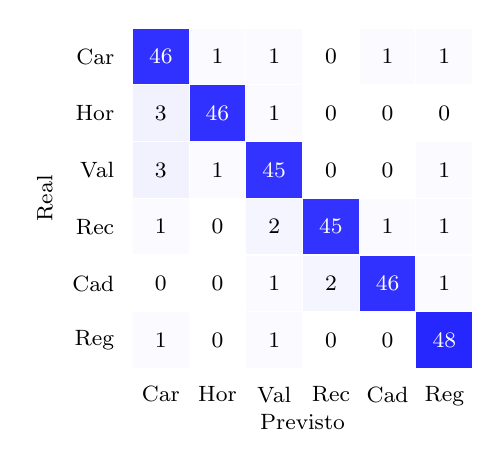
\begin{tikzpicture}[x=.72cm,y=.72cm,font=\footnotesize]
\filldraw[fill=blue!81,draw=white] (0,5) rectangle (1,6);
\node[text=white] at (0.5,5.5) {46};
\filldraw[fill=blue!2,draw=white] (1,5) rectangle (2,6);
\node[text=black] at (1.5,5.5) {1};
\filldraw[fill=blue!2,draw=white] (2,5) rectangle (3,6);
\node[text=black] at (2.5,5.5) {1};
\filldraw[fill=blue!0,draw=white] (3,5) rectangle (4,6);
\node[text=black] at (3.5,5.5) {0};
\filldraw[fill=blue!2,draw=white] (4,5) rectangle (5,6);
\node[text=black] at (4.5,5.5) {1};
\filldraw[fill=blue!2,draw=white] (5,5) rectangle (6,6);
\node[text=black] at (5.5,5.5) {1};
\filldraw[fill=blue!5,draw=white] (0,4) rectangle (1,5);
\node[text=black] at (0.5,4.5) {3};
\filldraw[fill=blue!81,draw=white] (1,4) rectangle (2,5);
\node[text=white] at (1.5,4.5) {46};
\filldraw[fill=blue!2,draw=white] (2,4) rectangle (3,5);
\node[text=black] at (2.5,4.5) {1};
\filldraw[fill=blue!0,draw=white] (3,4) rectangle (4,5);
\node[text=black] at (3.5,4.5) {0};
\filldraw[fill=blue!0,draw=white] (4,4) rectangle (5,5);
\node[text=black] at (4.5,4.5) {0};
\filldraw[fill=blue!0,draw=white] (5,4) rectangle (6,5);
\node[text=black] at (5.5,4.5) {0};
\filldraw[fill=blue!5,draw=white] (0,3) rectangle (1,4);
\node[text=black] at (0.5,3.5) {3};
\filldraw[fill=blue!2,draw=white] (1,3) rectangle (2,4);
\node[text=black] at (1.5,3.5) {1};
\filldraw[fill=blue!80,draw=white] (2,3) rectangle (3,4);
\node[text=white] at (2.5,3.5) {45};
\filldraw[fill=blue!0,draw=white] (3,3) rectangle (4,4);
\node[text=black] at (3.5,3.5) {0};
\filldraw[fill=blue!0,draw=white] (4,3) rectangle (5,4);
\node[text=black] at (4.5,3.5) {0};
\filldraw[fill=blue!2,draw=white] (5,3) rectangle (6,4);
\node[text=black] at (5.5,3.5) {1};
\filldraw[fill=blue!2,draw=white] (0,2) rectangle (1,3);
\node[text=black] at (0.5,2.5) {1};
\filldraw[fill=blue!0,draw=white] (1,2) rectangle (2,3);
\node[text=black] at (1.5,2.5) {0};
\filldraw[fill=blue!4,draw=white] (2,2) rectangle (3,3);
\node[text=black] at (2.5,2.5) {2};
\filldraw[fill=blue!80,draw=white] (3,2) rectangle (4,3);
\node[text=white] at (3.5,2.5) {45};
\filldraw[fill=blue!2,draw=white] (4,2) rectangle (5,3);
\node[text=black] at (4.5,2.5) {1};
\filldraw[fill=blue!2,draw=white] (5,2) rectangle (6,3);
\node[text=black] at (5.5,2.5) {1};
\filldraw[fill=blue!0,draw=white] (0,1) rectangle (1,2);
\node[text=black] at (0.5,1.5) {0};
\filldraw[fill=blue!0,draw=white] (1,1) rectangle (2,2);
\node[text=black] at (1.5,1.5) {0};
\filldraw[fill=blue!2,draw=white] (2,1) rectangle (3,2);
\node[text=black] at (2.5,1.5) {1};
\filldraw[fill=blue!4,draw=white] (3,1) rectangle (4,2);
\node[text=black] at (3.5,1.5) {2};
\filldraw[fill=blue!81,draw=white] (4,1) rectangle (5,2);
\node[text=white] at (4.5,1.5) {46};
\filldraw[fill=blue!2,draw=white] (5,1) rectangle (6,2);
\node[text=black] at (5.5,1.5) {1};
\filldraw[fill=blue!2,draw=white] (0,0) rectangle (1,1);
\node[text=black] at (0.5,0.5) {1};
\filldraw[fill=blue!0,draw=white] (1,0) rectangle (2,1);
\node[text=black] at (1.5,0.5) {0};
\filldraw[fill=blue!2,draw=white] (2,0) rectangle (3,1);
\node[text=black] at (2.5,0.5) {1};
\filldraw[fill=blue!0,draw=white] (3,0) rectangle (4,1);
\node[text=black] at (3.5,0.5) {0};
\filldraw[fill=blue!0,draw=white] (4,0) rectangle (5,1);
\node[text=black] at (4.5,0.5) {0};
\filldraw[fill=blue!85,draw=white] (5,0) rectangle (6,1);
\node[text=white] at (5.5,0.5) {48};
\node[anchor=north] at (0.5,-.15) {Car};
\node[anchor=north] at (1.5,-.15) {Hor};
\node[anchor=north] at (2.5,-.15) {Val};
\node[anchor=north] at (3.5,-.15) {Rec};
\node[anchor=north] at (4.5,-.15) {Cad};
\node[anchor=north] at (5.5,-.15) {Reg};
\node[anchor=east] at (-.15,5.5) {Car};
\node[anchor=east] at (-.15,4.5) {Hor};
\node[anchor=east] at (-.15,3.5) {Val};
\node[anchor=east] at (-.15,2.5) {Rec};
\node[anchor=east] at (-.15,1.5) {Cad};
\node[anchor=east] at (-.15,0.5) {Reg};
\node at (3.0,-.95) {Previsto};
\node[rotate=90] at (-1.55,3.0) {Real};
\end{tikzpicture}\end{minipage}
